\subsection{Digitale filtre}
%Digitale filtre kan opnå tusinde gange bedre resultat end analoge filtre.

Digitale filtre benyttes grundlæggende til to formål; adskillelse og genskabelse af signaler. Signaladskillelse %benyttes til at adskille signaler fra hinanden, hvilket ofte 
benyttes ofte i forbindelse med at filtrere støj fra det ønskede signal.\fxnote{eksempelvis ved ekg eller hjertelyd, hvor vejrtrækning og andre kropssignaler/lyde skal fjernes} Signalgenskabelse benyttes, hvis signalet er blevet beskadiget eller forvrænget. \fxnote{eksempelvis ved rystelser hvis måleudstyret er dårligt eller hvis ikke vi får sat den ordentlig fast på forsøgspersonen.} \citep{Smith1997}

Ethvert lineært filter har en impulsrespons, steprespons og en frekvensrespons. Disse responser indeholder information om filteret på forskellig vis og giver tilsammen information om, hvordan filteret vil agerer i givne situationer.\fxnote{hvis en af disse er oplyst eller defineret for filteret, kan de to andre udregnes matematisk.} \citep{Smith1997} Et filter designes ud fra dets responser. Den mest ligetil metode kaldes filterkernen eller Finite Impulse Response (FIR) filtre, hvor signalets inputs summeres med filterets impulsrespons. En anden metode kaldes et rekursivt filter eller Infinite Impulse Response (IIR) filtre, hvor tidligere outputværdier benyttes sammen med inputtet. For at finde impulsresponsen for et rekursivt filter, indsendes en impuls som input i filtret, og impulsresponsen er outputtet. Denne impulsrespons består af en sum af sinuser, som eksponentielt falder i amplitude. Dette resulterer i, at impulsresponsen bliver uendelig lang. \citep{Smith1997,Blandford2013} \newline
Et filter kan derudover designes ved, at filtrets steprespons eller frekvensrespons sammenholdes med sin impulsrespons. Stepresponsen er integralet af impulsresponsen, som kan findes ved at indsende en stepbølge i filteret. Outputtet heraf vil være stepresponsen. Frekvensresponsen kan findes ved at finde den diskrete Fourier transformationen (DFT) eller Fast Fourier transformationen (FFT) af impulsresponsen. \citep{Smith1997} %Resultatet af filterdesignet er typisk en overføringsfunktion i z-donæmet\fxnote{frekvensdomænet}. Ud fra denne kan filteret analyseres med henblik på at bestemme impulsresponsen, filterets stabilitet, steady-state frekvensrespons, differensformlen og responsen til et arbitrært input. \citep{Blandford2013} %I designfasen for filtre, startes der med at blive set på signalets frekvensspektrum, hvorved det vælges om der er behov for et lavpas-, højpas-, båndstop- eller båndpasfilter, og hertil også knækfrekvenserne for dem. Ud fra signalets frekvens, vælges også samplingshastigheden i henhold til Nyquist\fxnote{2 gange signalets frekvens}. Herefter vælges hvilken filtertype der egner sig bedst til systemet. \citep{Blandford2013}

\subsubsection{Finite Impulse Response filtre}
FIR filtre er defineret som digitale filtre med et endeligt antal impulsresponser. Det vil sige, at filteret har en impulsrespons med et endeligt antal ikke-nulværdier\fxnote{nonzeros}, hvorfor filtret kan designes stabilt og med en lineær fase. \citep{Blandford2013} Det fremgår af den generelle formel for FIR filtre, som ses i \eqref{eq:fir}, at filteret benytter tidligere og nutidige inputs. Dette er den afgørende faktor for, at responsen har et endeligt antal impulsresponser. 
\space
\begin{flalign}
	Y[n] = \sum_{m=0}^{m} b_m X[n-m]
	\label{eq:fir}
\end{flalign}
\space
FIR filtre inddeles i fire typer impulsresponsfunktioner, som det ses på \figref{fig:FIR_typer}. Type 1 har en lige orden og ulige længde, hvilket medfører, at responsen er centreret omkring den midterste impuls. Denne type er symmetrisk, hvorfor hele impulsresponsen ligger på den samme side af x-aksen. Type 2 er ligeledes symmetrisk, men har en ulige orden og lige længde. Dette resulterer i, at responsen er centreret imellem de to midterste impulser. %Disse kan skrives som en sum af cosinus funktioner.
Type 3 har en lige orden og ulige længde men er asymmetrisk, hvilket %i modsætning til type 1 og 2, 
gør at impulsresponsen ligger på begge sider af x-aksen. Type 4 har %, ligeledes med type 2, 
en ulige orden og lige længde, men er også asymmetrisk. %Disse kan skrives som en sum af sinus funktioner.
\citep{Blandford2013} \newline

\begin{figure}[H]
	\centering
	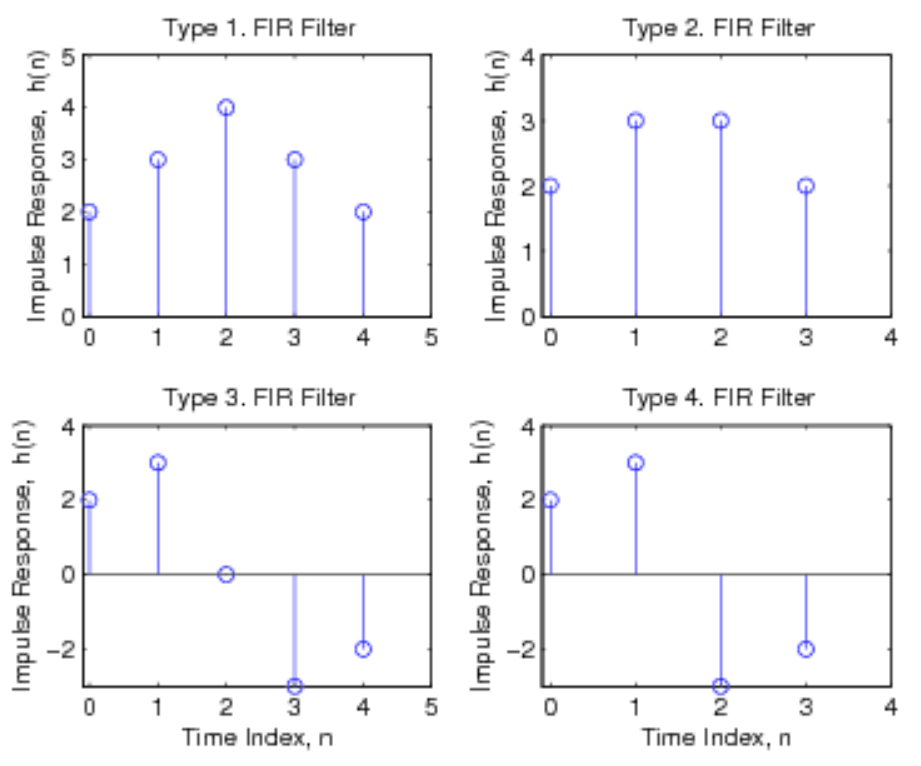
\includegraphics[scale=0.6]{figures/bProblemloesning/FIR_type.png}
	\caption{På figuren ses de fire typer af FIR filtre der finders. Yderligere illustreres ordenen, længden og symmetrien for de fire typer filtre. \citep{Burrus2016}}
	\label{fig:FIR_typer}
\end{figure}

De forskellige impulsresponsfunktioner benyttes til valg af filtertype, hvor det vurderes, hvilke der egner sig bedst til formålet. De forskellige konfigurationer skal tage højde for, om der ønskes et lavpas-, højpas-, båndpas- eller båndstopfilter. \citep{Blandford2013} \newline
FIR filtre optræder ligeledes som forskellige konfigurationer, heriblandt Parks-McClellan algoritmen, frekvens sampling, window type og moving average. \citep{Blandford2013}
%
%Windowing:
%Når der benyttes Fourier serier til at lave et ideelt FIR filter, fås en række koefficienter mellem minus uendelig og plus uendelig. Da et uendelig langt filter ikke kan implementeres, forkortes antallet af koefficienter til et antal som kan implementeres og stadig tilnærmelsesvis giver et ideelt filter. Matematisk sker dette ved at gange impulsresponsen med et rektangulært window. 
%
%Diskret fourier transformation (DFT) af et rektangulært window i tidsdomænet, giver en sinusfunktion i frekvensdomænet.
%
%\begin{flalign}
%Y[n] = H*W = \sum_{k=0}^{\infty} H[k] \cdot W[n-k]
%\label{eq:window}
%\end{flalign}
%
%
%Derudover kan filtrene implementeres på forskellig vis, alt efter deres formål. Moving average filtre benyttes til at udglatte signalet, ved at finde gennemsnitsværdien for et bestemt antal samples. Herved får en eventuel støj får mindre betydning for signalets udformning.
%
%\begin{flalign}
%	avg = \frac{1}{N} \sum_{i=1}^{N} x_i
%	\label{eq:mavg}
%\end{flalign}


\subsubsection{Infinite Impulse Response filtre}
Et IIR filter er, modsat FIR filtre, defineret som et digitalt filter med uendelig mange impulsresponser. Derfor har dette filter en impulsrespons med uendeligt mange nulværdier\fxnote{zeros}, hvilket gør at filterets impulsresponsen falder eksponentielt i amplitude og resulterer i en uendelig respons. Filteret kan derfor kun tilnærmelsesvis designes med en lineær fase, hvorfor det kan risikere at være ustabilt. Idet IIR filtre benytter tidligere outputs, er det et feedback filter, hvilket gør det udregningseffektivt.\fxnote{nemmere at udregne} \citep{Blandford2013} Af den generelle formel for IIR filtre i \eqref{eq:iir} fremgår det, at filteret benytter tidligere og nutidige inputs men også tidligere outputs, hvormed det får uendeligt mange impulsresponser. 
\space
\begin{flalign}
	Y[n] = \sum_{k=1}^{k} a_k Y[n-k] + \sum_{m=0}^{m} b_m X[n-m]
	\label{eq:iir}
\end{flalign}
\space 
IIR filtre optræder som forskellige filterkonfigurationer, heriblandt Butterworth, Chebyshev og elliptisk. Disse kan alle benyttes til lavpas-, højpas-, båndpas- eller båndstopfilter og designes ud fra krav om ripples, linearitet, dæmpningsgrad og faseforskydelse. \citep{Blandford2013}